\documentclass[10pt]{beamer} 
     \hypersetup{pdfpagemode=FullScreen} 
     \usepackage{tikz} 
     \usetikzlibrary{shadows,patterns,shapes} 
     \usetikzlibrary{shapes.arrows,chains} 
     % serifenfreier Font -- fuer Praesentation geeignet/er 
     \listfiles % damit im Log alle benutzten Pakete aufgelistet werden 
     \usetheme[progressbar=frametitle]{metropolis} 
     \usepackage{appendixnumberbeamer} 
     \usepackage{booktabs} 
     \usepackage[scale=2]{ccicons} 
     \usepackage[utf8]{inputenc} 
     \usepackage{pgfplots} 
     \usepgfplotslibrary{dateplot} 
     \usepackage[ngerman]{babel} 
     \usepackage{xspace} 
     \usebackgroundtemplate{
     \tikz[overlay,remember picture] 
     \node[opacity=0.3, at=(current page.south east),anchor=south east,inner sep=0pt] {
     
\includegraphics[width=100mm]{./PDFcreater/Pictures/background.png}};
     } 
     %\usebackgroundtemplate{
\includegraphics[,right]{./PDFcreater/Pictures/background.png}}
     \definecolor{Purple}{HTML}{6D087C}
     \definecolor{Orange}{HTML}{CF4A30}
     
     % Theme colors are derived from these two elements
     \setbeamercolor{alerted text}{fg=Orange}
     
     % ... however you can of course override styles of all elements 
     \setbeamercolor{frametitle}{bg=Purple}
     
     \title{SolidEdge Feedback der Studierenden} 
     \begin{document} 
     \maketitle 
\begin{frame}[fragile]{Benoetigte_Stundenzahl_vom_gesamten_CAD_Kurs_pro_Woche} 
 \begin{figure}
 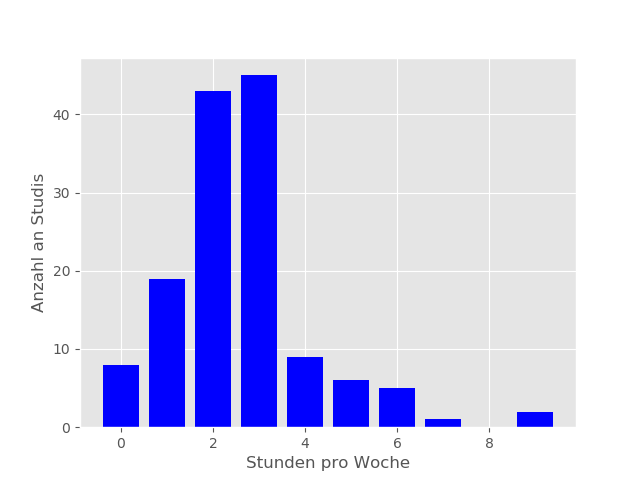
\includegraphics[width= 0.9\linewidth]{./PDFcreater/Plots/Benoetigte_Stundenzahl_vom_gesamten_CAD_Kurs_pro_Woche.png};
 \end{figure}
 \end{frame}
\begin{frame}[fragile]{Der_Lehrinhalt_war_ausreichend_um_die_HA_zu_bearbeiten} 
 \begin{figure}
 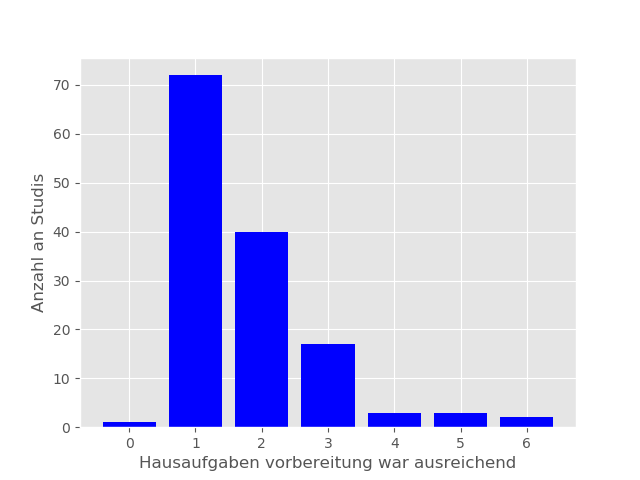
\includegraphics[width= 0.9\linewidth]{./PDFcreater/Plots/Der_Lehrinhalt_war_ausreichend_um_die_HA_zu_bearbeiten.png};
 \end{figure}
 \end{frame}
\begin{frame}[fragile]{Der_Schwierigkeitsgrad_war_hoch} 
 \begin{figure}
 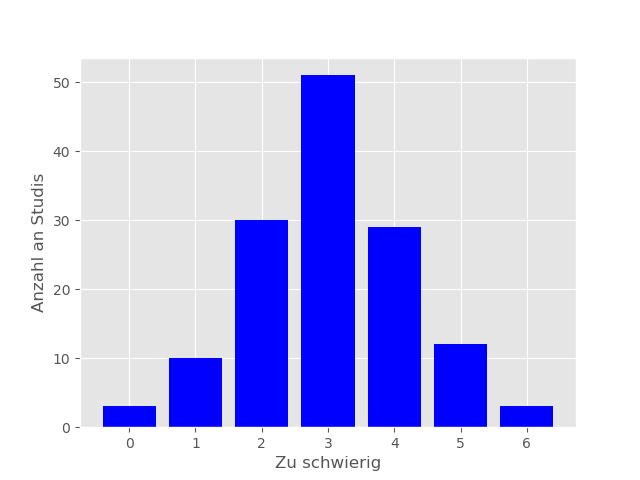
\includegraphics[width= 0.9\linewidth]{./PDFcreater/Plots/Der_Schwierigkeitsgrad_war_hoch.png};
 \end{figure}
 \end{frame}
\begin{frame}[fragile]{Die Formulierungen in der Hausaufgabe waren eindeutig} 
 \begin{figure}
 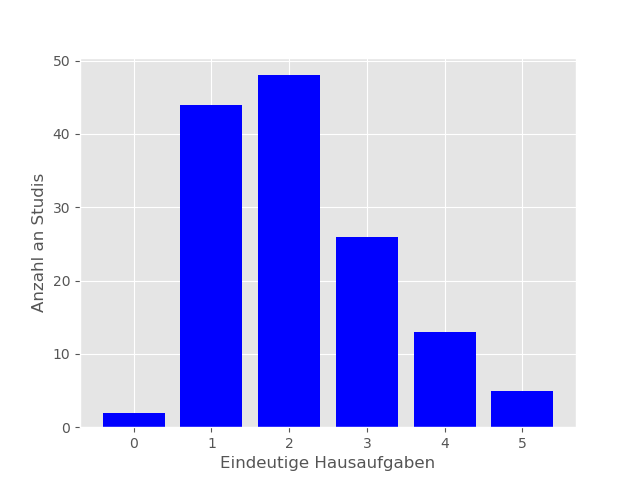
\includegraphics[width= 0.9\linewidth]{./PDFcreater/Plots/Die Formulierungen in der Hausaufgabe waren eindeutig.png};
 \end{figure}
 \end{frame}
\begin{frame}[fragile]{Die_Hausaufgabe_sollte_vom_Umfang_her_reduziert_werden} 
 \begin{figure}
 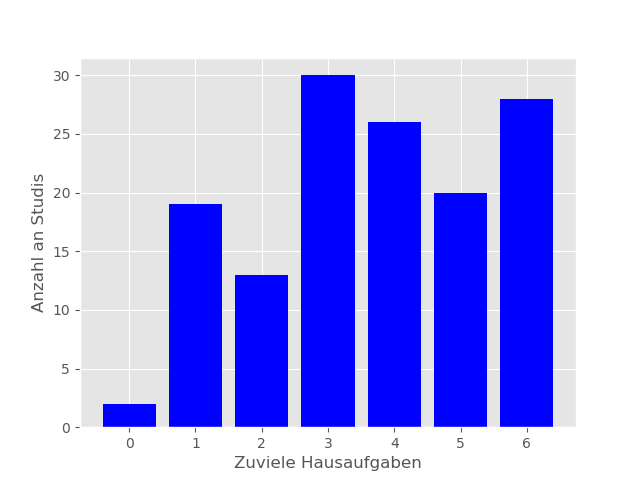
\includegraphics[width= 0.9\linewidth]{./PDFcreater/Plots/Die_Hausaufgabe_sollte_vom_Umfang_her_reduziert_werden.png};
 \end{figure}
 \end{frame}
\begin{frame}[fragile]{Die_Uebungen_sind_gut_strukturiert} 
 \begin{figure}
 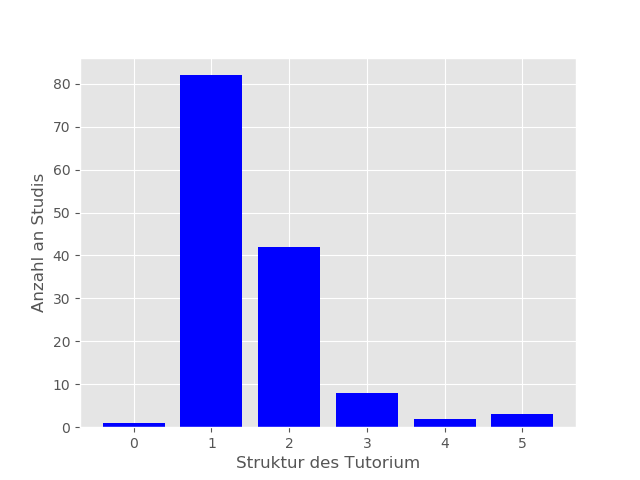
\includegraphics[width= 0.9\linewidth]{./PDFcreater/Plots/Die_Uebungen_sind_gut_strukturiert.png};
 \end{figure}
 \end{frame}
\begin{frame}[fragile]{Die_Uebungsbeispiele_sind_gut_gewaehlt} 
 \begin{figure}
 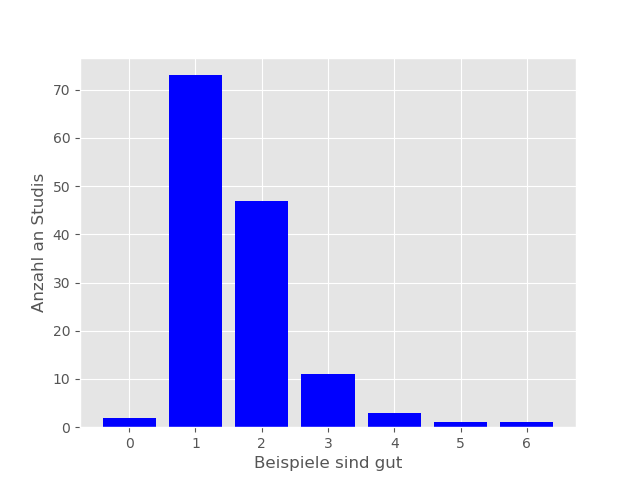
\includegraphics[width= 0.9\linewidth]{./PDFcreater/Plots/Die_Uebungsbeispiele_sind_gut_gewaehlt.png};
 \end{figure}
 \end{frame}
\begin{frame}[fragile]{Geschlecht_der_Studis} 
 \begin{figure}
 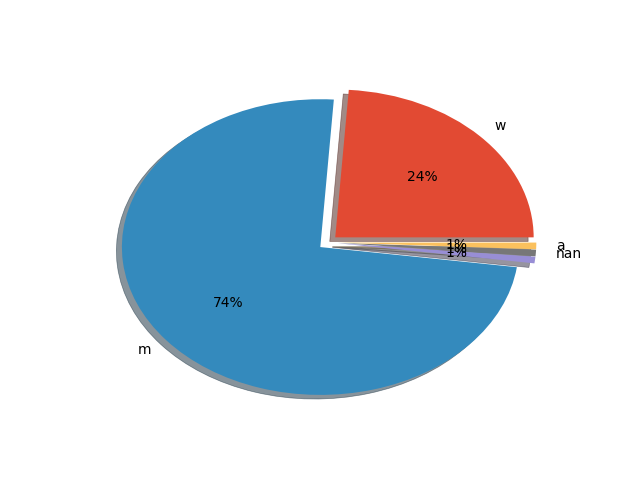
\includegraphics[width= 0.9\linewidth]{./PDFcreater/Plots/Geschlecht_der_Studis.png};
 \end{figure}
 \end{frame}
\begin{frame}[fragile]{Ich_habe_die_Uebungsaufgaben_alle_gemacht} 
 \begin{figure}
 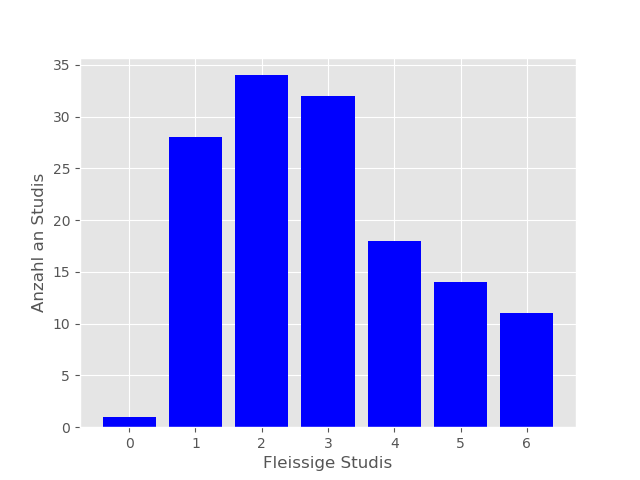
\includegraphics[width= 0.9\linewidth]{./PDFcreater/Plots/Ich_habe_die_Uebungsaufgaben_alle_gemacht.png};
 \end{figure}
 \end{frame}
\begin{frame}[fragile]{Ich_habe_mich_schon_fruehzeitig_mit_dem_Programm_zu_Hause_beschaeftigt} 
 \begin{figure}
 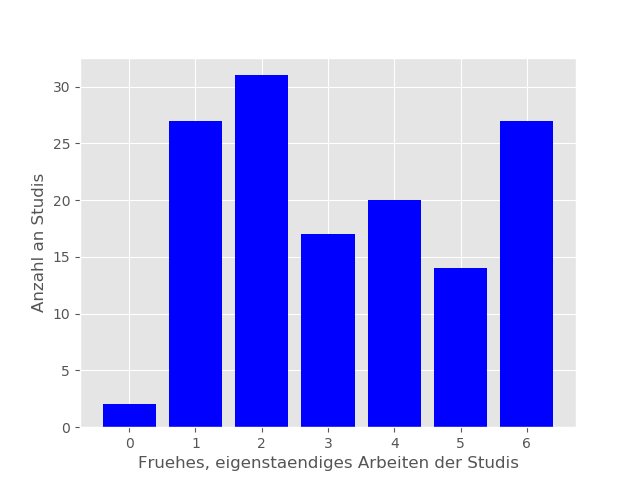
\includegraphics[width= 0.9\linewidth]{./PDFcreater/Plots/Ich_habe_mich_schon_fruehzeitig_mit_dem_Programm_zu_Hause_beschaeftigt.png};
 \end{figure}
 \end{frame}
\begin{frame}[fragile]{Ich_habe_viel_Zeit_zur_Bearbeitung_der_Hausaufgabe_benoetigt} 
 \begin{figure}
 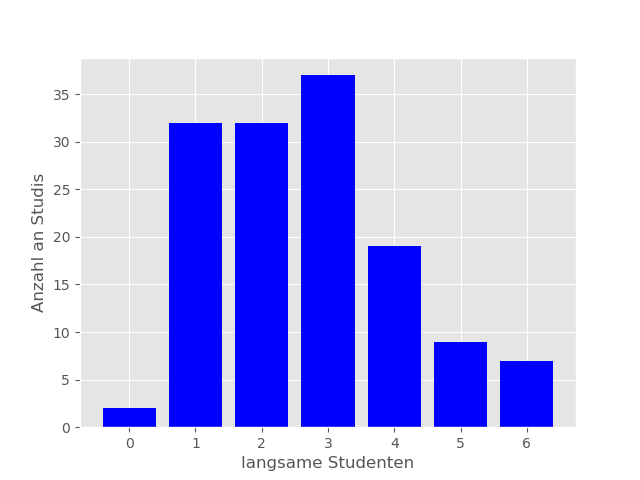
\includegraphics[width= 0.9\linewidth]{./PDFcreater/Plots/Ich_habe_viel_Zeit_zur_Bearbeitung_der_Hausaufgabe_benoetigt.png};
 \end{figure}
 \end{frame}
\begin{frame}[fragile]{Ich_haette_gerne_mehr_Uebungsaufgaben_gehabt} 
 \begin{figure}
 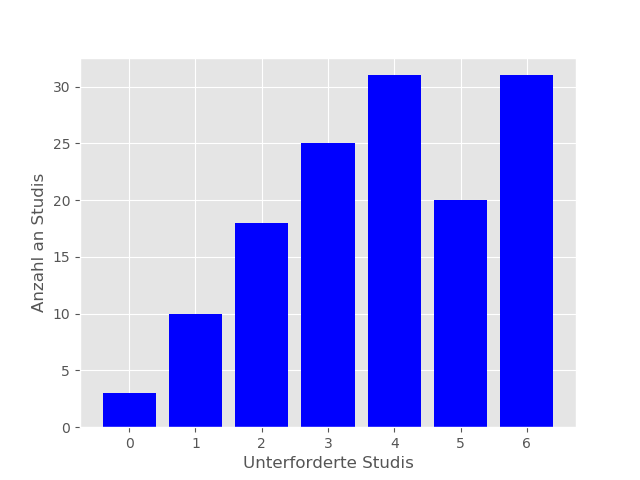
\includegraphics[width= 0.9\linewidth]{./PDFcreater/Plots/Ich_haette_gerne_mehr_Uebungsaufgaben_gehabt.png};
 \end{figure}
 \end{frame}
\begin{frame}[fragile]{Ich_war_immer_gut_auf_das_Tutorium_vorbereitet} 
 \begin{figure}
 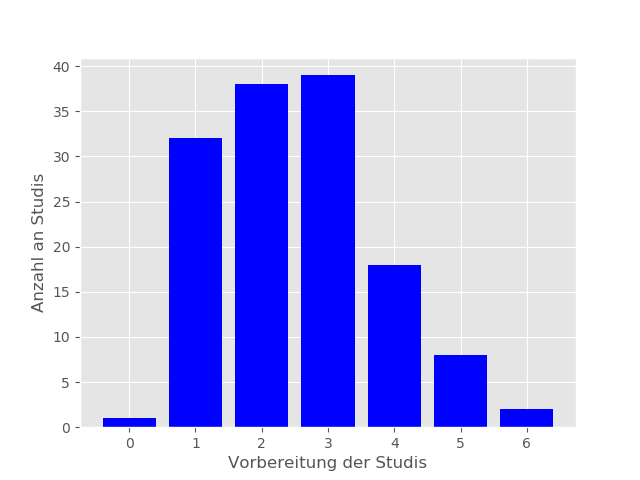
\includegraphics[width= 0.9\linewidth]{./PDFcreater/Plots/Ich_war_immer_gut_auf_das_Tutorium_vorbereitet.png};
 \end{figure}
 \end{frame}
\begin{frame}[fragile]{Semester_der_Studierenden} 
 \begin{figure}
 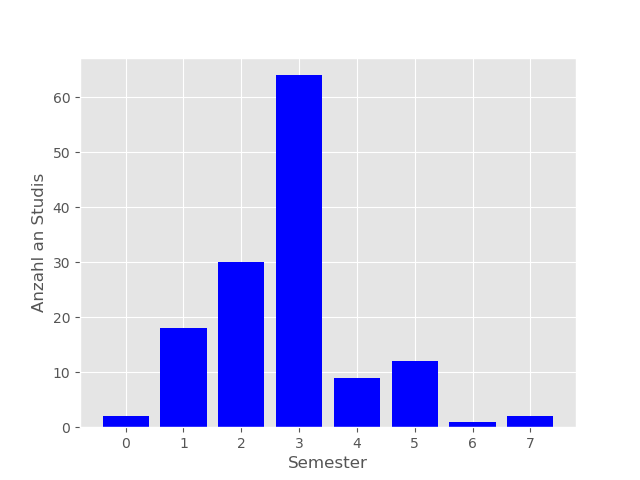
\includegraphics[width= 0.9\linewidth]{./PDFcreater/Plots/Semester_der_Studierenden.png};
 \end{figure}
 \end{frame}
\begin{frame}[fragile]{Studiengang_der_Studis} 
 \begin{figure}
 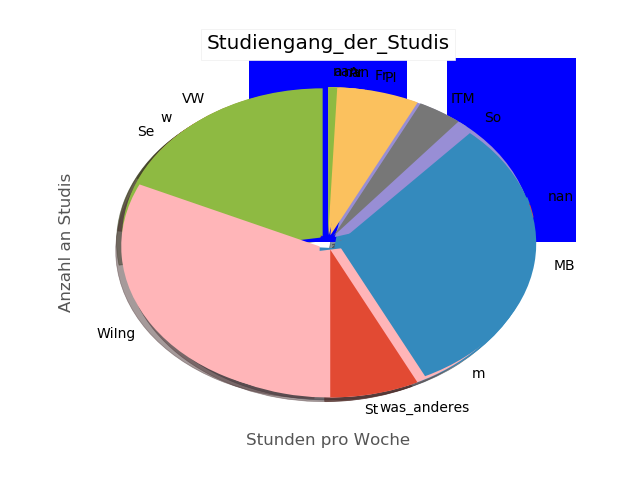
\includegraphics[width= 0.9\linewidth]{./PDFcreater/Plots/Studiengang_der_Studis.png};
 \end{figure}
 \end{frame}
\begin{frame}[fragile]{Tutor_der_Studis} 
 \begin{figure}
 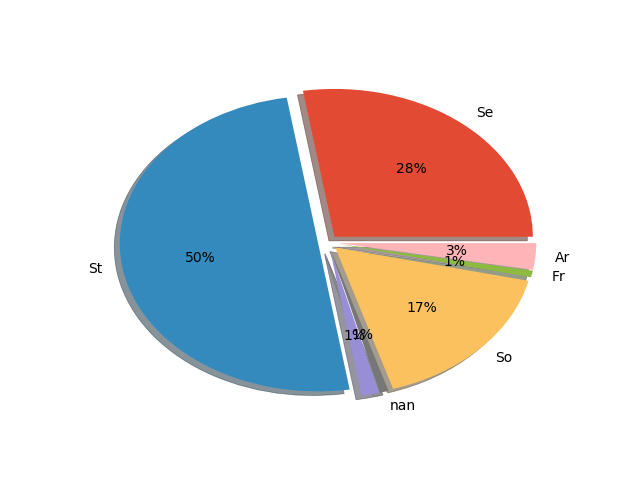
\includegraphics[width= 0.9\linewidth]{./PDFcreater/Plots/Tutor_der_Studis.png};
 \end{figure}
 \end{frame}
\begin{frame}[fragile]{Tutor_foerdert_aktive_Teilnahme_der_Studenten} 
 \begin{figure}
 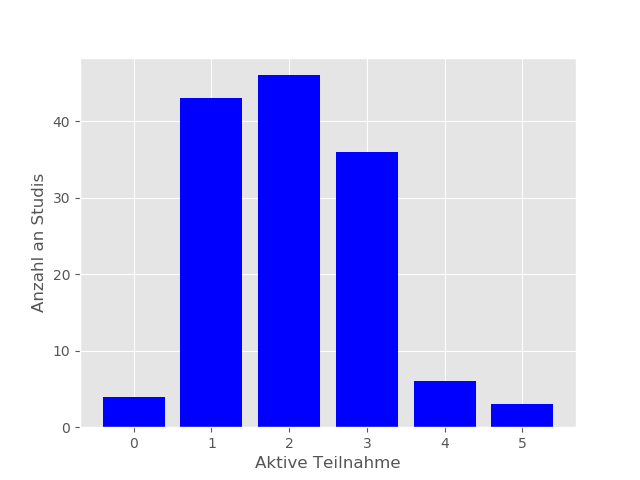
\includegraphics[width= 0.9\linewidth]{./PDFcreater/Plots/Tutor_foerdert_aktive_Teilnahme_der_Studenten.png};
 \end{figure}
 \end{frame}
\begin{frame}[fragile]{Tutor_ist_immer_gut_auf_das_Tutorium_vorbereitet} 
 \begin{figure}
 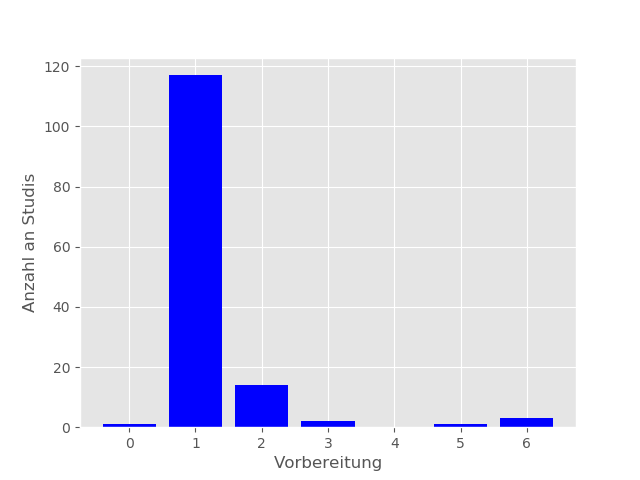
\includegraphics[width= 0.9\linewidth]{./PDFcreater/Plots/Tutor_ist_immer_gut_auf_das_Tutorium_vorbereitet.png};
 \end{figure}
 \end{frame}
\begin{frame}[fragile]{Tutor_kann_den_Lehrinhalt_verstaendlich_darlegen} 
 \begin{figure}
 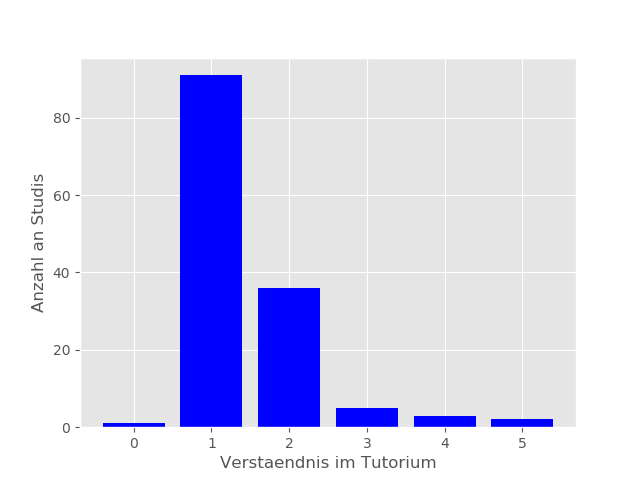
\includegraphics[width= 0.9\linewidth]{./PDFcreater/Plots/Tutor_kann_den_Lehrinhalt_verstaendlich_darlegen.png};
 \end{figure}
 \end{frame}
\end{document}